
\chapter{Metodologia}

Para responder as perguntas introduzidas na seção anterior, foi realizada uma pesquisa qualitativa através de entrevistas semi-estruturadas utilizando como base o roteiro desenvolvido pelo artigo base \cite{empiricalStudy2016}. A primeira seção abordará uma visão geral sobre os primeiros passos da pesquisa.  Já a segunda seção discorre sobre como as entrevistas foram conduzidas. Na terceira, encontra-se todo o processo utilizado para a análise dos dados obtidos na entrevista. Por último, a quarta seção mostra informações a respeito dos participantes da pesquisa.


\section{Pré-estudo}

Com o objetivo de entender melhor sobre como as práticas de CI/CD migraram para as empresas sediadas em Recife, essa fase do estudo contou com a participação de um segundo pesquisador para discussão do artigo base \cite{empiricalStudy2016}. Na discussão foi definido que seria aplicado apenas o estudo baseado em entrevistas semi-estruturadas para garantir o entendimento dos termos pelos entrevistados e a adequação com as definições do artigo base. 

Após a discussão, os pesquisadores acessaram o apêndice do trabalho para obter o guia de entrevista utilizado. Como forma de manter a consistência, foi utilizado o mesmo guia de entrevistas, assim como as mesmas definições utilizadas pelos autores. No início foi montado um arquivo com a definição de cada um dos termos envolvidos em língua portuguesa para ser utilizado como consulta caso haja alguma dúvida de definição de tópicos entre os entrevistadores.

Após isso, o guia de entrevistas do estudo base também foi traduzido para português e utilizado durante as entrevistas. Um ponto importante a respeito da tradução é o fato de que alguns termos ainda foram mantidos na língua inglesa devido ao fato de serem conhecidos mundialmente nesta língua. Por exemplo, \emph{Continuous Integration}, \emph{Canary Releases} e \emph{Health check}. O questionário utilizado está presente no \hyperlink{questionario}{apêndice A} deste trabalho em sua versão traduzida.

\section{Estrutura da Entrevista}

O guia de entrevistas se baseia na estratégia de evitar perguntas diretas (exemplo: “determinada prática está sendo utilizada?”). Esse modelo é essencial para garantir que a comparação entre participantes a respeito do uso ou não de práticas está sendo feita de maneira concisa, e não baseada nos conhecimentos prévios de cada participante. Assim, através de perguntas sobre o processo utilizado pelo entrevistado é possível, com uma certa margem de erro associada, afirmar que práticas ele utiliza. A margem de erro surge do fato de o autor ter que refletir sobre as informações recebidas e as definições para inferir o uso ou não de certa prática.

A entrevista é dividida em 5 sessões: 

\begin{enumerate}
\item Processo de entrega no geral
\item Papéis/Responsabilidades
\item Garantia da Qualidade (Quality Assurance)
\item Gerenciamento de Problemas
\item Avaliação de Entrega
\end{enumerate}

No guia, todas as sessões iniciam com uma questão aberta. As entrevistas seguiram os tópicos abordados em cada uma delas, mas sem ordem específica, respeitando o desenrolar da conversa. A primeira entrevista foi guiada pelos dois pesquisadores para assegurar que as próximas seriam feitas de forma semelhante pelos dois. Esta entrevista foi considerada como válida na análise de dados visto que não houve nenhuma mudança no questionário de entrevistas; o próprio já tinha sido validado no artigo utilizado de base para este trabalho. As outras 10 -- totalizando 11 entrevistas feitas -- foram guiadas por apenas um entrevistador, sendo 5 feitas por cada um dos dois pesquisadores.

Todas as entrevistas ocorreram de forma online, através do Google Meet, e aconteceram entre os meses de Setembro e Outubro de 2020 em português brasileiro. As entrevistas levaram entre 30 e 65 minutos, duração bem parecida com os tempos obtidos no artigo base (35 a 60 minutos), totalizando 7 horas e 15 minutos. Cada uma delas foi gravada pela plataforma para futura análise e 4 delas foram transcritas para o uso em citações neste trabalho, escolhidas através da relevância da entrevista e da forma como certos termos e processos foram apresentados pelo entrevistado. Foi deixado claro em cada uma das conversas a respeito da gravação e que estas seriam utilizadas apenas pelos entrevistadores, respeitando assim o anonimato do participante e confidencialidade de demais informações pessoais, bem como da empresa onde o participante trabalha.

\section{Participantes}

No total foram entrevistados 11 desenvolvedores (P1 a P11) de 7 empresas diferentes sediadas em Recife. A \figref{detalhamento_dos_entrevistados} mostra todos os dados demográficos obtidos de cada um dos entrevistados. Esses dados foram obtidos pelos entrevistadores no começo de cada entrevista e agregados nesta figura. O tamanho da empresa é definido pela quantidade de colaboradores: \emph{Startup} define empresas com menos de 50 trabalhadores; \emph{SME} são empresas que contém entre 50 e 500 colaboradores; e \emph{CORP} são empresas com mais de 500 colaboradores.


Da amostra, 3 eram mulheres. Pode-se ver a distribuição dos participantes por gênero na \figref{genero}. Dentro desse grupo, 9 trabalhavam com aplicações Web, enquanto 1 trabalhava com sistemas embarcados e o último, com jogos.

\begin{figure}[ht]
\begin{center}
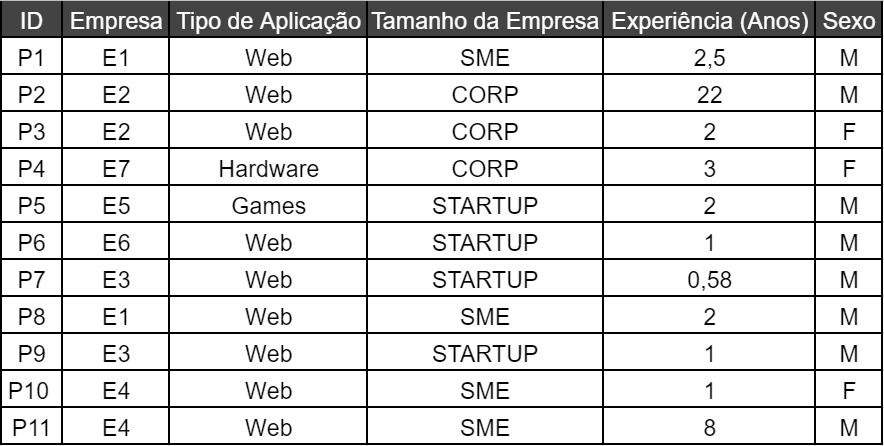
\includegraphics[scale=0.5]{detalhamento_dos_entrevistados.png}
\end{center}
\caption[Detalhamento dos entrevistados]{
    Detalhamento dos entrevistados da amostra, contendo todos os dados demográficos coletados.
}\label{detalhamento_dos_entrevistados}
\end{figure}


A escolha dos entrevistados foi feita baseado na rede de conhecidos dos entrevistadores, com o propósito de agregar pessoas que trabalhavam em empresas de tamanhos distintos para garantir uma variedade de parâmetros envolvidos. Como é possível perceber na \figref{tamanho_empresa}, com relação a esse aspecto a amostra está bem distribuída. 

\begin{figure}
\centering
\begin{minipage}{.48\textwidth}
    \centering
    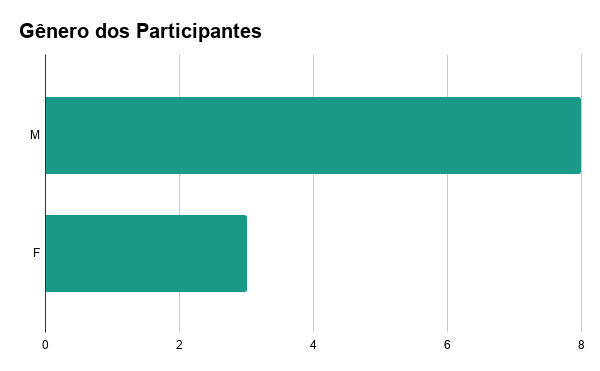
\includegraphics[scale=0.35]{demographics-genero.png}
    \caption[Distribuição dos Participantes por gênero]{
    Distribuição dos Participantes por gênero
    }\label{genero}
\end{minipage}%
\hfill
\begin{minipage}{.48\textwidth}
    \centering
    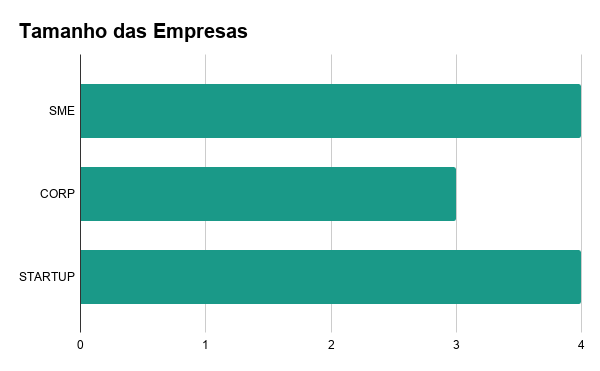
\includegraphics[scale=0.35]{demographics-tamanh-das-empresas.png}
    \caption[Distribuição dos Participantes por tamanho da empresa]{
    Distribuição dos Participantes por tamanho da empresa.
    }\label{tamanho_empresa}
\end{minipage}
\end{figure}

\section{Análise dos Dados}

\begin{figure}[ht]
\begin{center}
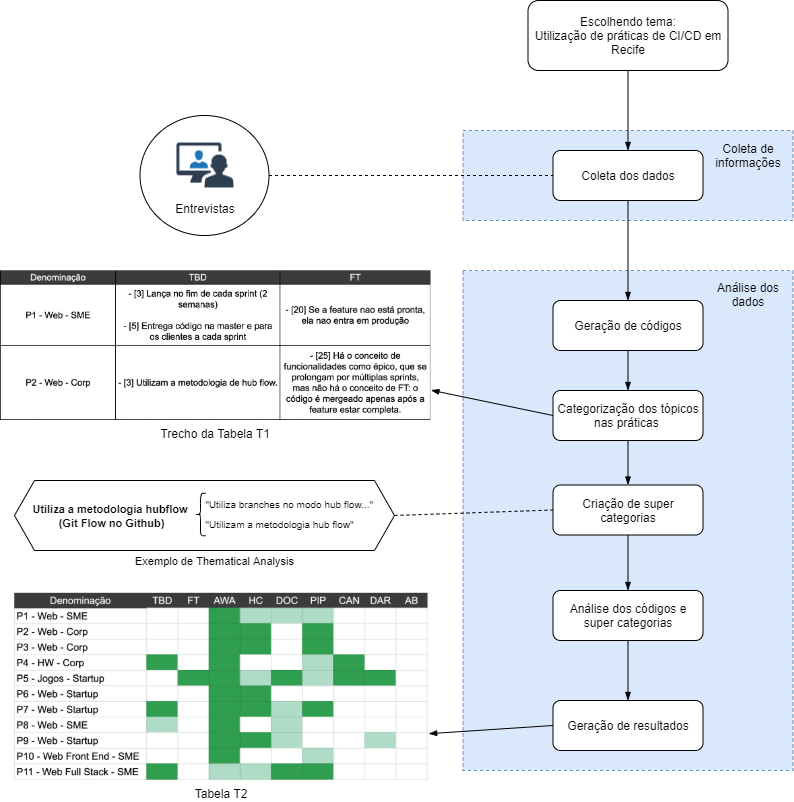
\includegraphics[scale=0.5]{metodologia_tcc.png}
\end{center}
\caption[Fluxograma da Metodologia]{
    Demonstra como funcionou os processos de coleta e análise de dados.
}\label{fluxograma_metodologia}
\end{figure}

    
A \figref{fluxograma_metodologia} apresenta uma visão geral de como funcionou o processo de coleta e análise de dados. A análise foi feita apenas pelo autor deste estudo. O processo escolhido foi baseado nas fases de \emph{Coding} e \emph{Thematic Analysis} da metodologia \emph{Grounded Theory} \cite{groundedTheory}. No processo de \emph{Coding} a ideia é levantar rótulos ou tags relevantes para o texto e, tradicionalmente, é feito baseado na transcrição das entrevistas. No entanto, neste trabalho o autor gerou códigos através da escuta das entrevistas. Então, como um exemplo, a seguinte citação:

\begin{quotation}[]{P5}
Como somos uma equipe muito pequena, todos os desenvolvedores são meio que DEVOPS. Quando tem que tomar alguma decisão nós entramos em discussão e definimos por nós.
\end{quotation}

Gerou o código: \emph{``Todos os desenvolvedores são devops.''} -- P5\_15, onde P5 identifica o número do participante do qual a entrevista gerou o código, e o 15 define a ordem de criação deste, além de servir como identificador único.

Então, após levantados todos os códigos de uma entrevista, estes foram revisados para garantir semântica e sintaxe adequadas. Alguns códigos nessa fase foram eliminados por redundância, enquanto outros foram quebrados em múltiplos. Depois, eles foram agrupados, quando compatíveis, em cada uma das 9 práticas descritas pelo artigo base e foi escolhida uma nota entre 0 a 2, representando não utiliza, utiliza parcialmente e utiliza completamente baseado nas definições do artigo base traduzidas. Por exemplo, na \figref{fluxograma_metodologia} pela etapa de ``Categorização dos tópicos nas práticas''. Este processo foi então replicado para cada uma das 11 entrevistas.

Ao final do processo ainda haviam 3 entrevistas que não geraram nenhum código relacionado a prática de \emph{Dark Launch}. Para estes casos, foi enviado um email diretamente para cada um dos entrevistados com a definição do artigo base da técnica e foi perguntado se o entrevistado utilizava ou não a mesma, o que gerou mais 3 códigos. Ao final, 292 códigos surgiram ao todo \footnote{A lista de todos os códigos está disponível em \url{http://bit.ly/tgMValgueiroCodigos}}.

Após a etapa de geração e revisão dos códigos, estes foram então agrupados, quando válido, na prática específica com a qual aquele código se relacionava. Este agrupamento gerou a Tabela Entrevistado-Pratica-Codigos, presente no \hyperlink{tabela1}{apêndice B} deste trabalho, que mostra uma visão geral de cada relação entre prática e entrevistado, contendo a nota dada e os códigos que justificam a nota. A nota é demonstrada pela cor presente em cada célula: branco significa não utiliza, verde claro mostra que o participante utiliza parcialmente, e verde mais escuro, totalmente. A tabela contém 147 dos 292 códigos gerados e foi utilizada como base para a maioria das figuras geradas neste trabalho. A \figref{trecho_tabela_t1} apresenta um trecho da Tabela Entrevistado-Pratica-Codigos.

\begin{figure}[ht]
    \begin{center}
    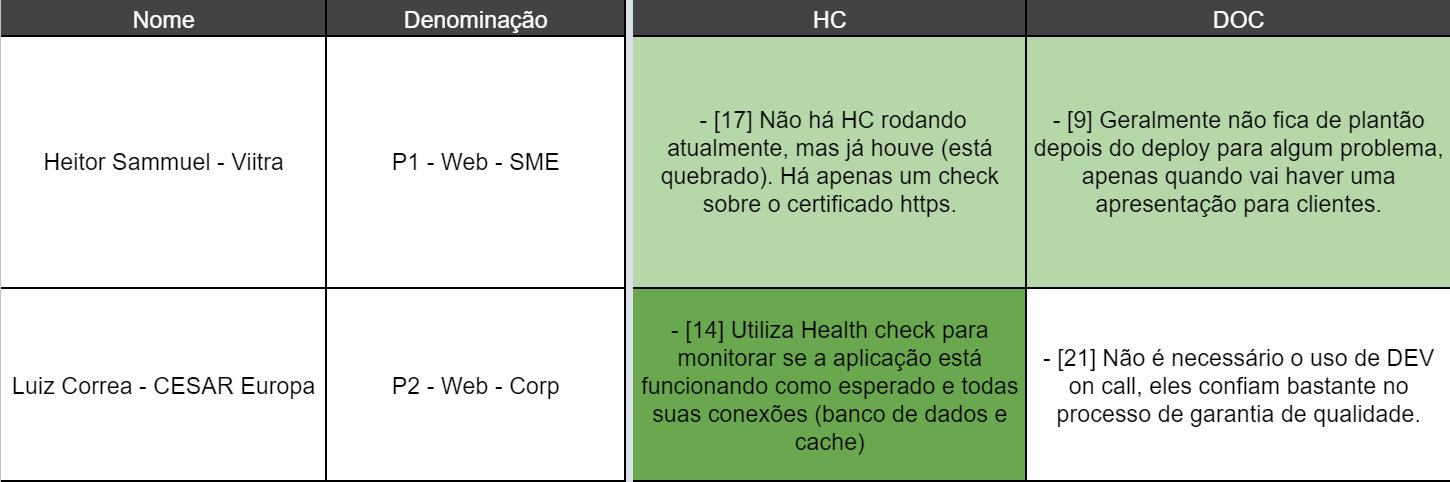
\includegraphics[scale=0.40]{tabelaT1-trecho-com-notas.png}
    \end{center}
    \caption[Trecho da Tabela Entrevistado-Pratica-Codigos]{
        Trecho da Tabela Entrevistado-Pratica-Codigos, com os códigos derivados das entrevistas agrupados por prática. As cores de cada célula representam a nota dada para determinada prática e foram dadas com base nos códigos presentes nela. Em algumas células há mais de uma evidência.
}\label{trecho_tabela_t1}
\end{figure}

Para identificar padrões e abstrações nos códigos agrupados na Tabela Entrevistado-Pratica-Codigos (\hyperlink{tabela1}{apêndice B}), foi feito um trabalho de agrupamento semântico, gerando por fim 17 novas super categorias através do processo de \emph{Thematic Analysis} \cite{groundedTheory}. Esse processo é ilustrado pela etapa de ``Criação de super categorias'' na \figref{fluxograma_metodologia}. As super categorias tinham como objetivo agrupar códigos semelhantes ou de mesma semântica para facilitar na reflexão dos dados. Um exemplo de super categoria gerada para a prática de \emph{Trunk Based Development} [TBD] pode ser encontrado na \figref{exemplo_super_categoria}. A tabela com todas as super categorias geradas pode ser encontrada no \hyperlink{super_Categorias}{Apêndice C}.

\begin{figure}[ht]
\begin{center}
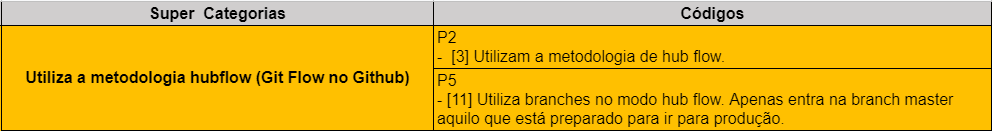
\includegraphics[width=\textwidth]{exemplo_super_categoria.png}
\end{center}
\caption[Exemplo de super categoria]{
    Exemplo de super categoria gerada durante o processo de \emph{Thematic Analysis}.
}\label{exemplo_super_categoria}
\end{figure}

É importante salientar que ainda durante o processo de levantamento de códigos surgiram tópicos relevantes que não se relacionavam diretamente com as práticas descritas, mas que são perguntados pelo questionário e relevantes para o tema tratado. Surgiram então 2 novos tópicos que agregam códigos sobre as práticas de \emph{Code Review} e de testes automáticos. Para estas foram relacionados 29 códigos dos 292 já mencionados, e duas super categorias foram geradas. A tabela com todos os códigos relacionados está presente no \hyperlink{tabela1}{apêndice B} juntamente com as outras práticas.

Por fim, foram geradas algumas tabelas derivadas da Tabela Entrevistado-Pratica-Codigos, ilustrado no passo de ``Geração de resultados'' na \figref{fluxograma_metodologia}, para facilitar a visualização e análise dos dados agregados, mostrando um mapa de utilização das práticas na amostra de diferentes formas. Essas tabelas serão apresentadas na próxima seção.
